\documentclass[12pt, a4paper]{article}

\usepackage[czech]{babel}
\usepackage{lmodern}
\usepackage[utf8]{inputenc}
\usepackage[T1]{fontenc}
\usepackage[pdftex]{graphicx}
\usepackage{amsmath, amssymb}
\usepackage[hidelinks,unicode]{hyperref}
\usepackage{float}
\usepackage{listings}
\usepackage{tikz}
\usepackage{xcolor}
\usepackage{tabularx}
\usepackage[final]{pdfpages}
\usepackage{syntax}
\usepackage{caption}
\usepackage{subcaption}
\usepackage{amsfonts}


\definecolor{mauve}{rgb}{0.58,0,0.82}
\usetikzlibrary{shapes,positioning,matrix,arrows}

\newcommand{\img}[1]{(viz obr. \ref{#1})}

\definecolor{pblue}{rgb}{0.13,0.13,1}
\definecolor{pgreen}{rgb}{0,0.5,0}
\definecolor{pred}{rgb}{0.9,0,0}
\definecolor{pgrey}{rgb}{0.46,0.45,0.48}


\lstdefinestyle{flex}{
    frame=tb,
    aboveskip=3mm,
    belowskip=3mm,
    showstringspaces=false,
    columns=flexible,
    basicstyle={\small\ttfamily},
    numbers=none,
    numberstyle=\tiny\color{black},
    keywordstyle=\color{black},
    commentstyle=\color{black},
    stringstyle=\color{black},
    breaklines=true,
    breakatwhitespace=true,
    tabsize=3
}

\lstset{
    frame=tb,
    language=C,
    aboveskip=3mm,
    belowskip=3mm,
    showstringspaces=false,
    columns=flexible,
    basicstyle={\small\ttfamily},
    numbers=none,
    numberstyle=\tiny\color{gray},
    keywordstyle=\color{blue},
    commentstyle=\color{pgreen},
    stringstyle=\color{mauve},
    breaklines=true,
    breakatwhitespace=true,
    tabsize=3
}


\let\oldsection\section
\renewcommand\section{\clearpage\oldsection}

\begin{document}
	% this has to be placed here, after document has been created
	% \counterwithout{lstlisting}{chapter}
	\renewcommand{\lstlistingname}{Ukázka kódu}
	\renewcommand{\lstlistlistingname}{Seznam ukázek kódu}
    \begin{titlepage}

        \centering

        \vspace*{\baselineskip}
        \begin{figure}[H]
        \centering
        
\includegraphics[width=7cm]{img/fav-logo.jpg}
        \end{figure}

        \vspace*{1\baselineskip}

        \vspace{0.75\baselineskip}

        \vspace{0.5\baselineskip}
        {Domácí úkol z předmětu KIV/VSS}

        {\LARGE\sc Generátory náhodných čísel\\}
        {\sc s Poissonovo rozdělením\\}

        \vspace{4\baselineskip}

        \vspace{0.5\baselineskip}

        {\sc\Large Stanislav Král \\}
        \vspace{0.5\baselineskip}
        {A20N0091P}

        \vfill

        {\sc Západočeská univerzita v Plzni\\
        Fakulta aplikovaných věd}

    \end{titlepage}

    % TOC
    \tableofcontents
    \pagebreak

\section{Zadání}
S využitím knihovní funkce pro generování pseudonáhodných čísel vytvořte generátor \textbf{Poissonovo} rozdělení jako funkci v jazyce Java, C, C++,Pascal/Delphi (kdy parametry rozdělení jsou zároveň parametry funkce generátoru) s využitím vhodné metody (inverzní transformace, kompoziční, vylučovací, atd.),

\section{Poissonovo rozdělení}
    Jedná se o rozdělení pravděpodobnosti, které popisuje diskrétní náhodnou veličinu vyjadřující počet výyskytů jevů v určitém intervalu, pokud jevy nastávají nezávisle na sobě a dílčí intervaly mezi jevy mají exponenciální rozdělení s parametrem 1.
Toto rozdělení se používá k aproximaci binomického rozdělení pro velký počet pokusů a malou pravděpodobnost výskytu sledovaného jevu v jednom pokusu.

    Jediným parametrem tohoto rozdělení je $\lambda$, který představuje střední hodnotu a rozptyl Poissonovo rozdělení. Tento parametr musí být z intervalu $(0, \infty)$.

     Diskrétní náhodná veličina $X$ se řídí Poissonovo rozdělením, pokud s použitím parametru $\lambda > 0$ má funkce hustoty pravděpodobnosti rozdělení následující tvar:
    \begin{displaymath}
       \!f(k; \lambda)= \Pr(X{=}k)= \frac{\lambda^k e^{-\lambda}}{k!}
    \end{displaymath}

    \begin{figure}[!ht]
        \centering
        \begin{minipage}{.5\textwidth}
            \centering
            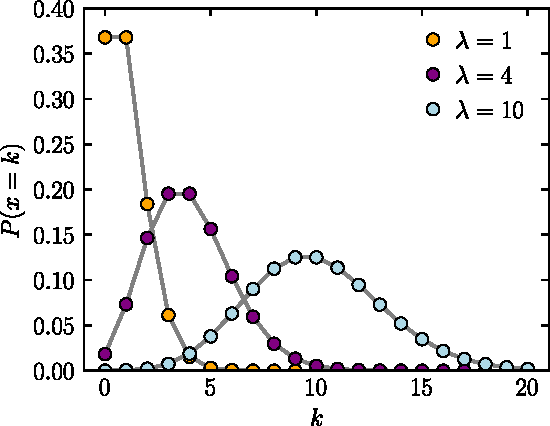
\includegraphics[width=.95\linewidth]{pdf/pmf.pdf}
            \captionof{figure}{Graf hustoty ppstní. funkce}
            \label{fig:test1}
        \end{minipage}%
        \begin{minipage}{.5\textwidth}
            \centering
            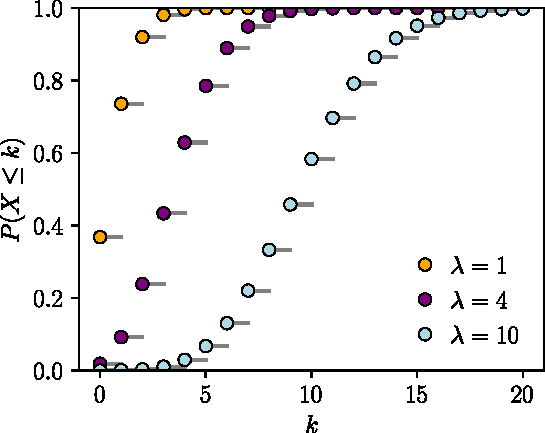
\includegraphics[width=.95\linewidth]{pdf/cdf.pdf}
            \captionof{figure}{Graf funkce rozdělení}
            \label{fig:test2}
        \end{minipage}
    \end{figure}

    Praktické využití Poissonova rozdělení lze pozorovat například při modelování vytížení telefonní ústředny, modelování rizika výskytu zemětřesení nebo modelování počtu fotonů dopadajících na teleskop\footnote{Rasch, Georg (1963), \hyperlink{http://www.rasch.org/memo1963.pdf}{"The Poisson Process as a Model for a Diversity of Behavioural Phenomena"} (PDF), 17th International Congress of Psychology, 2, Washington, DC, USA, August 20th – 26th, 1963: American Psychological Association}.

    \newpage
    \subsection{Střední hodnota}
    K odvození střední hodnoty Poissonova rozdělení s parametrem $\lambda$ lze použít následující postup:


    \begin{equation}
        \label{whatever}
        \begin{split}
        \mathbb{E}(X) &= \sum_{x \mathop \in X} x\,Pr(X = x) \\
        \mathbb{E}(X) & = \sum_{x=0}^{\infty}x\frac{\lambda^{x}}{x!}e^{-\lambda} \\
        & = \lambda\,e^{-\lambda}\sum_{x=0}^{\infty} \frac{\lambda^{x-1}}{(x-1)!} \\
        & = \lambda\,e^{-\lambda}e^{\lambda} \\
        & = \lambda
        \end{split}
    \end{equation}

    \subsection{Rozptyl}
    K odvození rozptylu Poissonova rozdělení s parametrem $\lambda$ lze použít následující postup\footnote{dle \url{https://proofwiki.org/wiki/Variance_of_Poisson_Distribution/Proof_1}}:

    \begin{equation}
        \label{whatever}
        \begin{split}
            var\,(X) & = \mathbb{E} (X^2) - (\mathbb{E} (X))^2 \\
            \mathbb{E} (X^2) &= \sum_{x \mathop \in \Omega_{X}} x^2 \, Pr(X = x) \\
            \mathbb{E} (X^2) &= \sum_{k \mathop \ge 0} {k^2 \dfrac 1 {k!} \lambda^k e^{-\lambda} } \\
            & = \lambda\, e^{-\lambda} \sum_{k \mathop \ge 1} {k \dfrac 1 {(k - 1)!} \lambda^{k - 1} } \\
            & = \lambda\, e^{-\lambda} ( \sum_{k \mathop \ge 1} {(k - 1) \dfrac 1 {(k - 1)!} \lambda^{k - 1} } + \sum_{k \mathop \ge 1} {\frac 1 {(k - 1)!} \lambda^{k - 1} }  ) \\
            & = \lambda\, e^{-\lambda} ( \lambda \sum_{k \mathop \ge 2} {\dfrac 1 {(k - 2)!} \lambda^{k - 2} } + \sum_{k \mathop \ge 1} {\dfrac 1 {(k - 1)!} \lambda^{k - 1} } ) \\
            & = \lambda\, e^{-\lambda} ( \lambda \sum_{i \mathop \ge 0} {\dfrac 1 {i!} \lambda^i} + \sum_{j \mathop \ge 0} {\dfrac 1 {j!} \lambda^j} ) \\
            & = \lambda\, e^{-\lambda} ( \lambda e^\lambda + e^\lambda) \\
            & = \lambda\, e^{-\lambda} ( \lambda e^\lambda + e^\lambda) \\
            & = \lambda^2 + \lambda \\
            var\,(X) & = \lambda^{2} + \lambda - \lambda^{2} = \lambda \\
        \end{split}
    \end{equation}



\end{document}    
